\section*{Результаты}
\subsection*{Решение двумерной задачи}

Для сравнения полученных результатов использовано эталонное решение из статьи \cite{2DBench}. 

\begin{table}[htp]
\center
  \begin{tabular}{lcccc}
\hline
	Re = 1000 
		& $\psi$   	& $\omega$ 	& x 		& y \\
\hline	
	Benchmark 	& 0.118942 	& 2.067213 	& 0.5300   	& 0.5650 \\
	Present		& 0.11523	& 2.06984	& 0.539		& 0.563 \\
\hline 
\hline
	Re = 5000 
		& $\psi$   	& $\omega$ 	& x 		& y \\
\hline	
	Benchmark 	& 0.122233 	& 1.940732 	& 0.5150   	& 0.5433 \\
	Present		& 0.1236	& 1.9387	& 0.514		& 0.550 \\
\hline 
  \end{tabular}
\caption{Занчения максимума функции тока $\psi$, значение завихренности $\omega$ в той же точке, и координаты этой точки для представленного 
метода (Present) и этолонного решения (Benchmark) \cite{2DBench}. При Re = 1000 и Re = 5000}
\label{comp}
\end{table}



\begin{figure}[htp]
\centering
\includegraphics[width = 1\linewidth]{resultImg/1000.pdf}
\caption{Изображены с лева на право функция тока, завизренность и поле давления. Re=1000}
\label{Re1000}
\end{figure}

\begin{figure}[htp]
\centering
\includegraphics[width = 1\linewidth]{resultImg/5000.pdf}
\caption{Изображены с лева на право функция тока, завизренность и поле давления. Re=5000}
\label{Re5000}
\end{figure}

На графиках \ref{Re1000},\ref{Re5000} изображена структура стационарного течения при Re=1000 и Re=5000. В правом и левом нижних углах существуют обратные вихри.  

\subsection*{Решение линеаризованной системы} 

Спектральная задача \ref{spactralProblem} зависит от двух параметров. Это число Рейнольдса Re и волновое чисо $\alpha$. Для каждой пары (Re,$\alpha$) может быть вычислен спектр задачи $\sigma(\Re,\alpha)$. Вычислив действительную часть каждого собственного значения в спектре и найдя среди них наименьшую найдем декримент затухания d(Ra,$\alpha$)
\begin{gather}
 d(\Re,\alpha) = \min_{\lambda \in \sigma(\Re,\alpha)} \mathfrak{R}(\lambda)
\end{gather}
Здесь $\mathfrak{R}$ обозначает реальную часть числа. Пусть дикременту соответствует множество собственных чисел $\Lambda_d$, вообще говоря, включающее только один элемент.
\begin{gather}
 \Lambda_d(\Re,\alpha) = \{ \lambda \in \sigma(\Re,\alpha) \mid d = \mathfrak{R}(\lambda) \}
\end{gather}
Составим еще одно множество $V_d$ из собственных векторов, соотвтствующих собственным значниям из определенного выше множества. Решение эволюционной задачи можно представить, как линейную комбинацию решений виде 
\begin{gather}
 V_\lambda e^{-\lambda t}
\end{gather}
Здесь $V_\lambda$ - собственный вектор, соответствующий собственному значению $\lambda$. 
По истечению некоторого времени каждым слагаемым, кроме того, собственное значение которого из
множества $\Lambda_d$, можно будет принебрачь. Если d больше нуля, решения устойчево, если d 
меньше нуля, решение неустойчево. Если в множестве $\Lambda_d$ всего одно значение $\lambda_d$, то 
решение будет асцелировать с частотой $\frac{\mathfrak{I}(\lambda_d)}{2\pi}$, где 
$\mathfrak{I}$~--- мнимая часть числа. Значния $d, V_d, \mathfrak{I}(\lambda_d)$ можно найти 
прямым численным интегрирование задачи \ref{iii}, не решая задачи на собственные значения.



Для каждого $\alpha$ можно вычислить критическое число Рейнольдся, обозначаемое $\Re_{crit}$, как наименьшее число Рейнольдся, при котором задача теряет устойчивость к возмущениям с длиной волны $\alpha$.
\begin{gather}
 \Re_{crit}(\alpha) = inf\{Re>0 \mid d(\Re,\alpha) < 0\}
\end{gather}
Кривую Re$_{crit}(\alpha)$ назавем \textit{кривой нейтральной стабильности}. Она определна на плоскости $(\Re,\alpha)$ при $\alpha > 0$. Во всех точках, лежищих ниже кривой,~--- задача устойчива к малым возмущениям. 

В реальном мире, конечно, возмущения развиваются произвольные, что значит, что начальные условия не нуливые при любом волновом числе. \textit{Глобальное критическое число Рейнольдса} $\Re_{crit}^*$, параметр исследуемой формы каверны, вычисляется как глобальный минимум кривой нейтральной устойчивости. Если при некотором числе Рейнольдся хотябы при одном значении волнового числа возмущения наростают, то есть дикримент отрицательный, течение не устойчиво к возмущениям. Если $R^+$~--- множество положительных рациональных чисел, то
\begin{gather}
 \Re_{crit}^* = \min_{\alpha \in R^+}(\Re_{crit}(\alpha))
\end{gather}

При равенстве волнового числа нулю, трехмерная задача эквивалентна двумерной исходной задаче. В этом случае $\Re_{crit}(0)$~--- число Рейнольдса, при котором двумерная задача теряет устойчивость к двумерным возмущениям. При числах Рейнольдса, меньших критического, в двумерной каверне существует двумерное стационарное течение. В статье \cite{lin-stability} представленно значение 8045.  

Расчет проводился при значениях числа рейнольдса от 100 до 5000, изменяющегося с шагом 50, и значениях волнового числа от 1 до 20, изменяющихся с шагом 1. Если решать задачу при каждом значении числа Рейнольдса и волнового числа, всего нужно провести 2000 испытвний. Для того, что бы число испытаний уменьшить, был использован следующий алгоритм. Для нахождения $Re_{crit}(\alpha)$ используется значение $\Re_{crit}(\alpha - \Delta\alpha)$. Вычисляется $d = d(\Re_{crit}(\alpha - \Delta\alpha), \alpha)$ если d > 0, вычисляем новое значение d при увеличеном на $\Delta \Re$ числе ренольдся, если d < 0~--- уменьшаем Re на $\Delta \Re$. Так, пока не будет найдено новое критическое сило рейнольдся. 
Таким образом можно сократить число испытвний, примерно, до 60. 

Численное решение спектральной задачи требует большого объема памяти и уже на сетках $50 \times 50$ памяти персонального компьютера не достаточно для расчета. Такой сетки достаточно лишь для чисел Рейнольдса, меньших 150. Для других чисел Рейнольдса, когда решить спектральную задачу не представляется возможным, линеаризованная система уравнений \ref{} интегрируется по времени до установления коэфициента затухания к значению дикремента. Так же, при Re < 150, результаты, полученный прямым численным интегрированием и из решения спектрильной задачи, можно сравить для проверки правельности програмной реализации и теоретических выкладок, что было успешно сделано. 
В таблтце \ref{Re_al} представленны результаты расчета в старвнении с результатами, получанными в \cite{lin-stability}. При $\alpha = 15$ значение $\Re_{crit}$ было вычисленно более точно, как как в этой точке достигается манимум.

\begin{table}[htp]
 \begin{tabular}{cccccc}
\hline
\hline
  \multicolumn{3}{c}{Бифуркация Андронова--Хопфа} & \multicolumn{3}{c}{Стационарные бифуркации} \\
  $\alpha$&	$\Re_{crit}(\alpha)$ \cite{lin-stability}&  Пр.&	$\alpha$&	$\Re_{crit}(\alpha)$ \cite{lin-stability}&  Пр. \\
\hline
  1&	8047&		-&	12&	925&		950\\ 
  2&	8046.6&		-&	13&	837.69&		850\\
  3&	4772.68&	4800&	14&	799.3&		800\\
  4&	4769.25&	4800&	15&	786&		790\\
  5&	1967.9&		1950&	16&	786&		790\\
  6&	1032&		1050&	17&	795.74&		800\\
  7&	932.5&		950&	18&	811.92&		850\\
  8&	939&		950&	19&	832.58&		850\\
  9&	1029.8&		1050&	20&	856&		900\\
  10&	1132&		1150\\
  11&	1040&		1050\\
\hline
 \end{tabular}
 \caption{Зависимость критического числа Рейнольдса от волнового числа. Для сравнения приведено решение из \cite{lin-stability}. }
 \label{Re_al}
\end{table}

\begin{figure}
  \center
  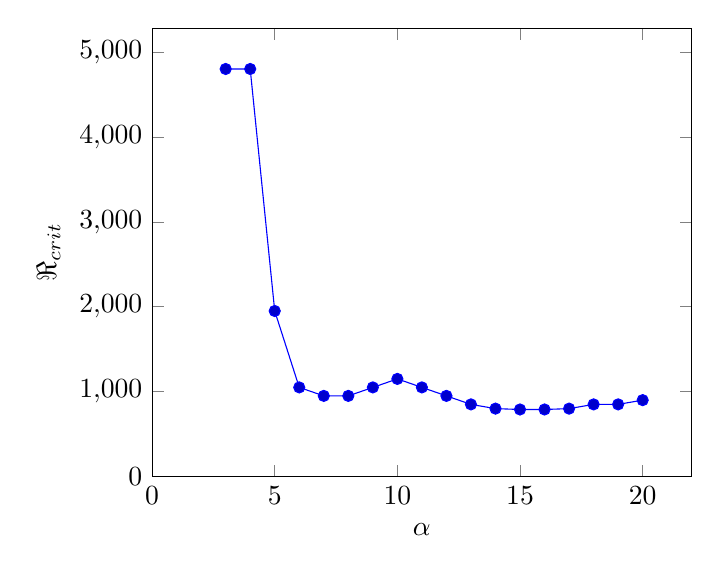
\begin{tikzpicture}
    \begin{axis}[
% 	xmode = log, ymode = log,
	xmin = 0, ymin = 0,
	xlabel=$\alpha$,
	ylabel=$\Re_{crit}$ ]
      \addplot coordinates {
	(3, 4800) (4, 4800) (5, 1950) (6, 1050) (7, 950) (8, 950) (9, 1050) (10, 1150)
	(11, 1050) (12, 950) (13, 850) (14, 800) (15, 790) (16, 790) (17, 800) (18, 850)
	(19, 850) (20, 900)};
    \end{axis}
  \end{tikzpicture}
  
  \caption{Кривая нейтральной стабильности}
  \label{graph:Re_al}
\end{figure}

Так же кривая нейтральной стабильности изображена на графике \ref{graph:Re_al}. Кривая имеет два локальных минимума. Первый~--- при $\alpha \approx 7 $. В этой точке реализуется бифуркация Андронова--Хопфа. Второй~--- при $\alpha \approx 15$. В этой точке реализуется стационарная бифуркация. В таблице данные разделены на две колонки, в соответствии с двумя механизмами возникновения неустоияивости.  Значения, достигаемые впервом и во втором локальных минимумах сравнимы между собой, но при этом голобальный минимум достикается при $\alpha \approx 15$ и критическое число Рейнольдса в этой точке равно глобальному критическому числу Рейнольдся и равно $\Re_{crit}^* = \Re_{crit}(15) = 790$. 

При расчете трехмерного течения нужны более плотные сетки по сравнению с расчетом двумерного течения \ref{2}. Под расчетом трехмерного течения понимается, как прямой расчет линеаризованной системы уравнений \ref{3}, так и решение собственной задачи \ref{4}. На одной и той же сетке оба метода решают одну разностную задачу, и их решение должны совподать. Если, при Re=1000, для расчета \ref{2} достаточно $128 \times 128$, для расчета \ref{3,4} нужно от $196 \times 196$ узлов в сетке. Если, для решения задачи \ref{2} на сетке $196 \times 196$ при том же Re=1000 шаг по времени был выбран 0.01, для решения задачи \ref{3,4} необходимо шаг уменьшить, хотябы, до 0.002.  

\newpage
